\documentclass[12pt, leqno]{article} %% use to set typesize
\include{common}

\begin{document}

\hdr{2022-09-20}

\section{Least squares basics}

\begin{figure}
  \begin{center}
  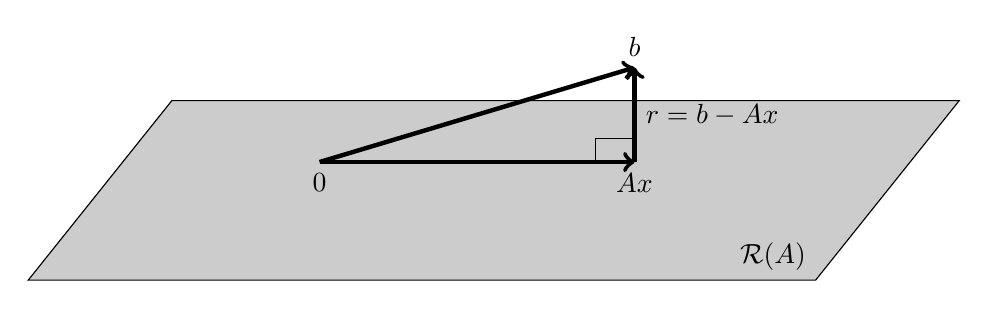
\begin{tikzpicture}
    \begin{scope}[xslant=0.8,xscale=5,yscale=3]
      \draw[fill=black!20] (-0.5,-0.5) rectangle (1.5,0.26);
      \draw[ultra thick,->]
        (0,0) node[below] {$0$} --
        (0.8,0) node[below] {$Ax$};
      \node[above left] at (1.5,-0.5) {$\mathcal{R}(A)$};
    \end{scope}
    \begin{scope}[xscale=5,yscale=3]
    \draw[ultra thick,->]
      (0,0) -- (0.8,0.4) node[above] {$b$};
    \draw[ultra thick,->]
      (0.8,0) -- (0.8,0.4) node[midway,right] {$r=b-Ax$};
    \draw (0.7,0) -- (0.7,0.1) -- (0.8,0.1);
    \end{scope}
  \end{tikzpicture}
  \end{center}
  \caption{Picture of a linear least squares problem.  The vector $Ax$
           is the closest vector in $\mathcal{R}(A)$ to a target
           vector $b$ in the Euclidean norm.  Consequently, the
           residual $r = b-Ax$ is normal (orthogonal) to
           $\mathcal{R}(A)$.}
  \label{fig1}
\end{figure}

A {\em least squares} problem involves minimization of a (squared)
Euclidean norm of some vector:
\[
  \mbox{minimize } \frac{1}{2} \|r\|^2 \mbox{ s.t. } r \in \Omega.
\]
In general, the derivative of the squared norm is given by
\[
  \delta \left( \frac{1}{2} \|r\|^2 \right) = \Re \langle \delta r, r \rangle;
\]
we will usually assume least squares problems over the real numbers,
in which case we don't have to worry about taking the real part.
If we want to minimize the Euclidean norm of $r$ (in the real case), we need
\[
  \langle \delta r, r \rangle = 0 \mbox{ for all admissible } \delta r;
\]
that is, $r$ is orthogonal (or normal) to any admissible variation
$\delta r$ at the point.  Here an ``admissible'' variation is just one
that we could produce by changing the system in an allowed way.

For example, consider $A \in \mathbb{R}^{m \times n}$ with $m > n$ and
let $r(x) = A x - b$.  This is a {\em linear least squares} problem.
In this setting, the admissible variations are $\delta r = A \delta
x$, and the first-order condition for a minimizer is
\[
  \forall \delta x \in \mathbb{R}^n, \langle A \delta x, Ax - b \rangle = 0.
\]
Using the standard inner product, this gives us
\[
  A^T (Ax - b) = A^T A x - A^T b = 0,
\]
which is sometimes known as the {\em normal equations} because the
residual is normal to all admissible variations (Figure~\ref{fig1}).

The normal equations have a unique solution when $A$ is full column
rank.  The solution to the normal equations is
\[
  (A^T A)^{-1} A^T b = A^\dagger b,
\]
where $A^\dagger = (A^T A)^{-1} A$ is the {\em Moore-Penrose pseudoinverse}
of $A$.  It is a pseudoinverse because $A^\dagger A = I$, but
$P = A A^\dagger$ is not an identity.  Instead, $P$ is a
{\em projector}, i.e.~$P^2 = P$.  We say $P$ is the orthogonal
projector onto $\mathcal{R}(A)$.  Conceptually, it maps each point to
the nearest point in the range space of $A$.  The projector $I-P$ is
the residual projector, for which $\mathcal{R}(A)$ is the null space.

If you are not entirely happy with the variational calculus argument,
there is a more algebraic approach.  We note that for
$x = A^\dagger b + z$
we have
\begin{align*}
  \|Ax-b\|^2
  &= \|Az-(I-P)b\|^2 \\
  &= \|Az\|^2 + \|(I-P)b\|^2
\end{align*}
by the Pythagorean theorem (since $Az \perp (I-AA^\dagger) b$ by the
normal equations).  When $A$ is full rank, positive definiteness
implies that $\|Az\|^2 > 0$ for $z \neq 0$; therefore, the minimizer
happens at $z = 0$.

An alternate formulation for the normal equations for the linear least
squares problem is
\[
  \begin{bmatrix} I & A \\ A^T & 0 \end{bmatrix}
  \begin{bmatrix} r \\ x \end{bmatrix} =
  \begin{bmatrix} b \\ 0 \end{bmatrix}
\]
where the first row in the system defines $r = b-Ax$ and the second
row gives the normal condition $A^T r = 0$. Partial Gaussian
elimination on this alternative system gives the normal equations
$A^T A x = A^T b$ as a Schur complement subsystem.

Nothing we have said is specific to the standard inner product.  If
$M$ is any symmetric positive definite matrix, there is an associated
inner product
\[
  \langle x, y \rangle_M = y^T M x,
\]
and we can write the normal equations in terms of this inner product:
\[
  A^T M (Ax - b) = 0.
\]
Similarly, we can generalize the alternative form of the least squares
problem to
\[
\begin{bmatrix} M^{-1} & A \\ A^T & 0 \end{bmatrix}
\begin{bmatrix} \tilde{r} \\ x \end{bmatrix} =
\begin{bmatrix} b \\ 0 \end{bmatrix}
\]
where $\tilde{r} = M r$ is the scaled residual.

\section{Minimum norm problems}

So far, we have considered overdetermined problems.  But it is also
interesting to consider minimum norm solutions to underdetermined
problems:
\[
  \mbox{minimize } \frac{1}{2} \|x\|^2 \mbox{ s.t. } Ax = b
\]
where $A \in \bbR^{m \times n}$ and now $m < n$.  In this case, using
the method of Lagrange multipliers, we have
\[
  \mathcal{L}(x, \lambda) = \frac{1}{2} \|x\|^2 + \lambda^T (Ax - b)
\]
and the stationary equations are
\[
0 = \delta \mathcal{L} =
  \delta x^T (x + A^T \lambda) + \delta \lambda^T (Ax-b)
\]
for all $\delta x$ and $\delta \lambda$.  Alternately, in matrix form,
we have
\[
  \begin{bmatrix} I & A^T \\ A & 0 \end{bmatrix}
  \begin{bmatrix} x \\ \lambda \end{bmatrix} =
  \begin{bmatrix} 0 \\ b \end{bmatrix}.
\]
Eliminating the $x$ variable gives us $(AA^T) \lambda = b$,
and back-substitution yields
\[
  x = A^T (A A^T)^{-1} b.
\]
When $A$ is short and wide rather than tall and skinny (and assuming
it is full row rank), we say that $A^\dagger = A^T (AA^T)^{-1}$ is the
Moore-Penrose pseudo-inverse.

\section{Why least squares?}

Why is the ordinary least squares problem interesting?
There are at least three natural responses.

\begin{enumerate}
  \item {\bf Simplicity:}
  The least squares problem is one of the simplest formulations
  around for fitting linear models.  The quadratic loss model
  is easy to work with analytically; it is smooth; and it leads
  to a problem whose solution is linear in the observation data.

  \item {\bf Statistics:}
  The least squares problem is the optimal approach to parameter
  estimation among linear unbiased estimators, assuming independent
  Gaussian noise.  The least squares problem is also the maximum likelihood
  estimator under these same hypotheses.

  \item {\bf It's a building block:}
  Linear least squares are not the right formulation for all regression
  problems --- for example, they tend to lack robustness in the face of
  heavy-tailed, non-Gaussian random errors.  But even for these cases,
  ordinary least squares is a useful {\em building block}.
  Because least squares problems are linear in the observation vector,
  they are amenable to direct attack by linear algebra methods in a way
  that other estimation methods are not.  The tools we
  have available for more complex fitting boil down to linear algebra
  subproblems at the end of the day, so it is useful to learn how to work
  effectively with linear least squares.
\end{enumerate}

\section{Least squares and statistical models}

Consider the model
\[
  y_i = \sum_{j=1}^n c_j x_{ij} + \epsilon_i
\]
where the {\em factors} $x_{ij}$ for example $j$ are known,
and the observations $y_i$ are assumed to be an (unknown)
combination of the factor values plus independent noise
terms $\epsilon_i$ with mean zero and variance $\sigma^2$.
In terms of a linear system, we have
\[
  y = X c + \epsilon.
\]

\subsection{Gauss-Markov}

A {\em linear unbiased estimator} for $c$ is a linear combination
of the observations whose expected value is $c$; that is, we
need a matrix $M \in \bbR^{n \times m}$ such that
\[
  \mathbb{E}[M y] = M X c = c.
\]
That is, $M$ should be a pseudo-inverse of $X$.  Clearly one choice of
linear unbiased estimator is $\hat{c} = X^\dagger y$.  According to
the Gauss-Markov theorem, this is actually the {\em best} linear
unbiased estimator, in the sense of miminizing the variance.  To see
this, consider any other linear unbiased estimator.  We can always
write such an estimator as
\[
  \tilde{c} = (X^\dagger + D) y
\]
where $D \in \bbR^{n \times m}$ satisfies $D X = 0$.  Then
\begin{align*}
  \operatorname{Var}(\tilde{c})
  &= \operatorname{Var}((X^\dagger + D) y) \\
  &= (X^\dagger + D) (\sigma^2 I) (X^\dagger D) \\
  &= \sigma^2 (X^\dagger + D) (X^\dagger + D)^T \\
  &= \sigma^2 (X^T X)^{-1} + \sigma^2 D D^T
  &= \operatorname{Var}(\hat{c}) + \sigma^2 D D^T,
\end{align*}
i.e. the variance of $\tilde{c}$ exceeds that of $\hat{c}$ by a
positive definite matrix.  And when the noise has covariance $C$, the best
linear unbiased estimator satisfies the generalized least squares problem
$X^T C^{-1} (Xc-y) = 0$ or, in alternate form
\[
  \begin{bmatrix} C & X \\ X^T & 0 \end{bmatrix}
  \begin{bmatrix} r \\ c \end{bmatrix} =
  \begin{bmatrix} y \\ 0 \end{bmatrix}.
\]

\subsection{Maximum likelihood}

Another estimator for the parameters $c$ in the model
$y = Xc + \epsilon$ comes from maximizing the (log) likelihood
function.  If $\epsilon$ is a vector of multivariate Gaussian noise
with mean zero and covariance $C$, then the likelihood function is
\[
  \ell(y) = \frac{1}{\sqrt{\det(2\pi C}} \exp\left( -\frac{1}{2} (y-Xc)^T C^{-1} (y-xC) \right),
\]
and for a fixed $C$, maximizing the likelihood corresponds to
minimizing $\|y-Xc\|_{C^{-1}}^2$.

Of course, Gaussian noise is not the only type of noise.  More general
noise models lead to more complex optimization problems.  For example,
if we assume the $\epsilon_i$ are Laplacian random variables (with
probability proportional to $\exp(-|z|)$ rather than $\exp(-z^2)$),
then maximizing the likelihood corresponds to maximimizing
$\|y-Xc\|_1$ instead of $\|y-Xc\|_2$.  This gives an estimator that is
a {\em nonlinear} function of the data.  However, least squares
computations can be used as a building block for computing this type
of estimators as well.

\subsection{Reasoning about the residual}

When we come to a least squares problem via a statistical model, it is
natural to check whether the residual terms behave as one might
expect:
\begin{itemize}
\item Are there about the same number of positive and negative
  residuals?
\item If there is a natural ``linear'' structure to the data, is there
  evidence of significant auto-correlation between consecutive
  residuals?
\item Does the residual behave like white noise, or does it
  concentrate on certain frequencies?
\end{itemize}
Even when they are small, residuals that do not appear particularly
noisy are a sign that the model may not describe the data particularly
well.

\section{A family of factorizations}

\subsection{Cholesky}

If $A$ is full rank, then $A^T A$ is symmetric and positive definite
matrix, and we can compute a Cholesky factorization of $A^T A$:
\[
  A^T A = R^T R.
\]
The solution to the least squares problem is then
\[
  x = (A^T A)^{-1} A^T b = R^{-1} R^{-T} A^T b.
\]
Or, in Julia world
\begin{lstlisting}
  F = chol(A'*A);
  x = F\(A'*b);
\end{lstlisting}

\subsection{Economy QR}

The Cholesky factor $R$ appears in a different setting as well.
Let us write $A = QR$ where $Q = AR^{-1}$; then
\[
  Q^T Q = R^{-T} A^T A R^{-1} = R^{-T} R^T R R^{-1} = I.
\]
That is, $Q$ is a matrix with orthonormal columns.  This
``economy QR factorization'' can be computed in several different
ways, including one that you have seen before in a different guise
(the Gram-Schmidt process).

Julia provides a numerically stable
method to compute the QR factorization via
\begin{lstlisting}
  F = qr(A)
\end{lstlisting}
and we can use the QR factorization directly to solve the least
squares problem without forming $A^T A$ by
\begin{lstlisting}
  F = qr(A)
  x = F\b
\end{lstlisting}
Behind the scenes, this is what is used when we write \verb|A\b| with
a dense rectangular matrix $A$.

\subsection{Full QR}

There is an alternate ``full'' QR decomposition where we write
\[
A = QR, \mbox{ where }
Q = \begin{bmatrix} Q_1 & Q_2 \end{bmatrix} \in \bbR^{n \times n},
R = \begin{bmatrix} R_{1} \\ 0 \end{bmatrix} \in \bbR^{m \times n}.
\]
To see how this connects to the least squares problem, recall
that the Euclidean norm is invariant under orthogonal transformations,
so
\[
  \|r\|^2 = \|Q^T r\|^2 = \left\| \begin{bmatrix} Q_1^T b \\ Q_2^T
    b \end{bmatrix} - \begin{bmatrix} R_1 \\ 0 \end{bmatrix} x
  \right\|^2 = \|Q_1^T b-R_1x\|^2 + \|Q_2^T b\|^2.
\]
We can set $\|Q_1^T v-R_1 x\|^2$ to zero by
setting $x = R_1^{-1} Q_1^T b$; the result is
$\|r\|^2 = \|Q_2^T b\|^2$.

The QR factorization routine in Julia can be used to reconstruct
either the full or the compact QR decomposition.  Internally, it
stores neither the smaller $Q_1$ nor the full matrix $Q$ explicitly;
rather, it uses a compact representation of the matrix as a product of
Householder reflectors, as we will discuss next time.

\subsection{SVD}

The full QR decomposition is useful because orthogonal transformations
do not change lengths.  Hence, the QR factorization lets us change
to a coordinate system where the problem is simple without changing
the problem in any fundamental way.  The same is true of the SVD,
which we write as
\begin{align*}
A &=
\begin{bmatrix} U_1 & U_2 \end{bmatrix}
\begin{bmatrix} \Sigma \\ 0 \end{bmatrix}
V^T & & \mbox{Full SVD} \\
&= U_1 \Sigma V^T & & \mbox{Economy SVD}.
\end{align*}
As with the QR factorization, we can apply an orthogonal
transformation involving the factor $U$ that makes the
least squares residual norm simple:
\[
\|U^T r\|^2 =
\left\| \begin{bmatrix} U_1^T b \\ U_2^T b \end{bmatrix} -
\begin{bmatrix} \Sigma V^T \\ 0 \end{bmatrix} x
\right\| =
\|U_1^T b - \Sigma V^T x\|^2 + \|U_2^T b\|^2,
\]
and we can minimize by setting $x = V \Sigma^{-1} U_1^T b$.

\end{document}
